\batchmode
\documentclass[twoside]{book}

% Packages required by doxygen
\usepackage{fixltx2e}
\usepackage{calc}
\usepackage{doxygen}
\usepackage[export]{adjustbox} % also loads graphicx
\usepackage{graphicx}
\usepackage[utf8]{inputenc}
\usepackage{makeidx}
\usepackage{multicol}
\usepackage{multirow}
\PassOptionsToPackage{warn}{textcomp}
\usepackage{textcomp}
\usepackage[nointegrals]{wasysym}
\usepackage[table]{xcolor}

% Font selection
\usepackage[T1]{fontenc}
\usepackage[scaled=.90]{helvet}
\usepackage{courier}
\usepackage{amssymb}
\usepackage{sectsty}
\renewcommand{\familydefault}{\sfdefault}
\allsectionsfont{%
  \fontseries{bc}\selectfont%
  \color{darkgray}%
}
\renewcommand{\DoxyLabelFont}{%
  \fontseries{bc}\selectfont%
  \color{darkgray}%
}
\newcommand{\+}{\discretionary{\mbox{\scriptsize$\hookleftarrow$}}{}{}}

% Page & text layout
\usepackage{geometry}
\geometry{%
  a4paper,%
  top=2.5cm,%
  bottom=2.5cm,%
  left=2.5cm,%
  right=2.5cm%
}
\tolerance=750
\hfuzz=15pt
\hbadness=750
\setlength{\emergencystretch}{15pt}
\setlength{\parindent}{0cm}
\setlength{\parskip}{3ex plus 2ex minus 2ex}
\makeatletter
\renewcommand{\paragraph}{%
  \@startsection{paragraph}{4}{0ex}{-1.0ex}{1.0ex}{%
    \normalfont\normalsize\bfseries\SS@parafont%
  }%
}
\renewcommand{\subparagraph}{%
  \@startsection{subparagraph}{5}{0ex}{-1.0ex}{1.0ex}{%
    \normalfont\normalsize\bfseries\SS@subparafont%
  }%
}
\makeatother

% Headers & footers
\usepackage{fancyhdr}
\pagestyle{fancyplain}
\fancyhead[LE]{\fancyplain{}{\bfseries\thepage}}
\fancyhead[CE]{\fancyplain{}{}}
\fancyhead[RE]{\fancyplain{}{\bfseries\leftmark}}
\fancyhead[LO]{\fancyplain{}{\bfseries\rightmark}}
\fancyhead[CO]{\fancyplain{}{}}
\fancyhead[RO]{\fancyplain{}{\bfseries\thepage}}
\fancyfoot[LE]{\fancyplain{}{}}
\fancyfoot[CE]{\fancyplain{}{}}
\fancyfoot[RE]{\fancyplain{}{\bfseries\scriptsize Generated by Doxygen }}
\fancyfoot[LO]{\fancyplain{}{\bfseries\scriptsize Generated by Doxygen }}
\fancyfoot[CO]{\fancyplain{}{}}
\fancyfoot[RO]{\fancyplain{}{}}
\renewcommand{\footrulewidth}{0.4pt}
\renewcommand{\chaptermark}[1]{%
  \markboth{#1}{}%
}
\renewcommand{\sectionmark}[1]{%
  \markright{\thesection\ #1}%
}

% Indices & bibliography
\usepackage{natbib}
\usepackage[titles]{tocloft}
\setcounter{tocdepth}{3}
\setcounter{secnumdepth}{5}
\makeindex

% Hyperlinks (required, but should be loaded last)
\usepackage{ifpdf}
\ifpdf
  \usepackage[pdftex,pagebackref=true]{hyperref}
\else
  \usepackage[ps2pdf,pagebackref=true]{hyperref}
\fi
\hypersetup{%
  colorlinks=true,%
  linkcolor=blue,%
  citecolor=blue,%
  unicode%
}

% Custom commands
\newcommand{\clearemptydoublepage}{%
  \newpage{\pagestyle{empty}\cleardoublepage}%
}

\usepackage{caption}
\captionsetup{labelsep=space,justification=centering,font={bf},singlelinecheck=off,skip=4pt,position=top}

%===== C O N T E N T S =====

\begin{document}

% Titlepage & ToC
\hypersetup{pageanchor=false,
             bookmarksnumbered=true,
             pdfencoding=unicode
            }
\pagenumbering{alph}
\pagenumbering{arabic}
\hypersetup{pageanchor=true}

%--- Begin generated contents ---
\chapter{Demo problem\+: 3D F\+SI on unstructured meshes}
\label{index}\hypertarget{index}{}\hypertarget{index_q}{}\section{A few quick questions...}\label{index_q}
Since {\ttfamily oomph-\/lib} is developed as open-\/source software, any evidence that the code is being downloaded and used is very helpful for us as it helps to justify our continued work on this project.

We would therefore be extremely grateful if you could provide the information requested in the form below. Pressing the \char`\"{}submit\char`\"{} button will get you to the actual download page.

{\bfseries Note\+:} 
\begin{DoxyItemize}
\item All information will be treated as confidential. 
\item If you provide your email address and check the appropriate box we will add you to our mailing list to inform you of upgrades and bug fixes to the code. Rest assured that the mailing list is {\bfseries very low volume} -- we have better things to do than to bombard you with email. 
\item If you still feel reluctant to provide any of the information requested, feel free to enter some dummy input. The form will check that {\bfseries some} information has been entered but entering your name as \char`\"{}\+Joe Cool\char`\"{} is perfectly acceptable -- this is to discourage people from not providing the information simply because they are too lazy to type... 
\end{DoxyItemize}



 







 

 \hypertarget{index_pdf}{}\section{P\+D\+F file}\label{index_pdf}
A \href{../latex/refman.pdf}{\tt pdf version} of this document is available. \end{document}

\chapter{Namespace Index}
\section{Namespace List}
Here is a list of all namespaces with brief descriptions\+:\begin{DoxyCompactList}
\item\contentsline{section}{\hyperlink{namespaceGlobal__Physical__Variables}{Global\+\_\+\+Physical\+\_\+\+Variables} \\*Global variables that represent physical properties }{\pageref{namespaceGlobal__Physical__Variables}}{}
\item\contentsline{section}{\hyperlink{namespaceoomph}{oomph} }{\pageref{namespaceoomph}}{}
\item\contentsline{section}{\hyperlink{namespacePhysical__Variables}{Physical\+\_\+\+Variables} \\*Namespace for the solution of 2D linear shell equation }{\pageref{namespacePhysical__Variables}}{}
\end{DoxyCompactList}

\chapter{Hierarchical Index}
\section{Class Hierarchy}
This inheritance list is sorted roughly, but not completely, alphabetically\+:\begin{DoxyCompactList}
\item Problem\begin{DoxyCompactList}
\item \contentsline{section}{Unstructured\+Solid\+Problem$<$ E\+L\+E\+M\+E\+NT $>$}{\pageref{classUnstructuredSolidProblem}}{}
\end{DoxyCompactList}
\end{DoxyCompactList}

\chapter{Class Index}
\section{Class List}
Here are the classes, structs, unions and interfaces with brief descriptions\+:\begin{DoxyCompactList}
\item\contentsline{section}{\hyperlink{classPMLProblem}{P\+M\+L\+Problem$<$ E\+L\+E\+M\+E\+N\+T $>$} }{\pageref{classPMLProblem}}{}
\item\contentsline{section}{\hyperlink{classGlobalParameters_1_1TestPMLMapping}{Global\+Parameters\+::\+Test\+P\+M\+L\+Mapping} }{\pageref{classGlobalParameters_1_1TestPMLMapping}}{}
\end{DoxyCompactList}

\chapter{File Index}
\section{File List}
Here is a list of all files with brief descriptions\+:\begin{DoxyCompactList}
\item\contentsline{section}{\hyperlink{jeffery__orbit_8cc}{jeffery\+\_\+orbit.\+cc} }{\pageref{jeffery__orbit_8cc}}{}
\item\contentsline{section}{\hyperlink{jeffery__orbit_8txt__doxygenified_8h}{jeffery\+\_\+orbit.\+txt\+\_\+doxygenified.\+h} }{\pageref{jeffery__orbit_8txt__doxygenified_8h}}{}
\item\contentsline{section}{\hyperlink{my__taylor__hood__elements_8h}{my\+\_\+taylor\+\_\+hood\+\_\+elements.\+h} }{\pageref{my__taylor__hood__elements_8h}}{}
\end{DoxyCompactList}

\chapter{Namespace Documentation}
\hypertarget{namespaceGlobal__Parameters}{}\section{Global\+\_\+\+Parameters Namespace Reference}
\label{namespaceGlobal__Parameters}\index{Global\+\_\+\+Parameters@{Global\+\_\+\+Parameters}}


Global variables.  


\subsection*{Functions}
\begin{DoxyCompactItemize}
\item 
void \hyperlink{namespaceGlobal__Parameters_a200109847bf4cc26da4d00e8d68d569e}{gravity} (const double \&time, const Vector$<$ double $>$ \&xi, Vector$<$ double $>$ \&b)
\begin{DoxyCompactList}\small\item\em Non-\/dimensional gravity as body force. \end{DoxyCompactList}\item 
double \hyperlink{namespaceGlobal__Parameters_a536aa5314a6cdb36af852e9513351d55}{flux} (const double \&t)
\begin{DoxyCompactList}\small\item\em Flux increases between Min\+\_\+flux and Max\+\_\+flux over period Ramp\+\_\+period. \end{DoxyCompactList}\item 
void \hyperlink{namespaceGlobal__Parameters_a8c333f9041cad78d5c0160a8e2c169f5}{set\+\_\+parameters} (const string \&case\+\_\+id)
\begin{DoxyCompactList}\small\item\em Set parameters for the various test cases. \end{DoxyCompactList}\end{DoxyCompactItemize}
\subsection*{Variables}
\begin{DoxyCompactItemize}
\item 
string \hyperlink{namespaceGlobal__Parameters_a887474a9be53363806b4de417f660dba}{Case\+\_\+\+ID} =\char`\"{}F\+S\+I1\char`\"{}
\begin{DoxyCompactList}\small\item\em Default case ID. \end{DoxyCompactList}\item 
double \hyperlink{namespaceGlobal__Parameters_a9d72e94a9305c6a310940a6a427ebe06}{Re} =20.\+0
\begin{DoxyCompactList}\small\item\em Reynolds number (default assignment for F\+S\+I1 test case) \end{DoxyCompactList}\item 
double \hyperlink{namespaceGlobal__Parameters_af1af40a0df651e86bc1be273fafa98da}{St} =0.\+5
\begin{DoxyCompactList}\small\item\em Strouhal number (default assignment for F\+S\+I1 test case) \end{DoxyCompactList}\item 
double \hyperlink{namespaceGlobal__Parameters_a7a59a32365e87566069e458dc83bd18a}{Re\+St} =10.\+0
\begin{DoxyCompactList}\small\item\em Product of Reynolds and Strouhal numbers (default assignment for F\+S\+I1 test case) \end{DoxyCompactList}\item 
double \hyperlink{namespaceGlobal__Parameters_a7814fddf663e56168174a42d2cd6b4c1}{Q} =1.\+429e-\/6
\begin{DoxyCompactList}\small\item\em F\+SI parameter (default assignment for F\+S\+I1 test case) \end{DoxyCompactList}\item 
double \hyperlink{namespaceGlobal__Parameters_a517d4c31b8bce6563c2f605266dd9679}{Density\+\_\+ratio} =1.\+0
\begin{DoxyCompactList}\small\item\em Density ratio (solid to fluid; default assignment for F\+S\+I1 test case) \end{DoxyCompactList}\item 
double \hyperlink{namespaceGlobal__Parameters_ab360628e7830e43e355ce5768f6d6a6c}{H} =0.\+2
\begin{DoxyCompactList}\small\item\em Height of flag. \end{DoxyCompactList}\item 
double \hyperlink{namespaceGlobal__Parameters_a0f0247cc83ba202413b50e7b4b7fceb0}{Centre\+\_\+x} =2.\+0
\begin{DoxyCompactList}\small\item\em x position of centre of cylinder \end{DoxyCompactList}\item 
double \hyperlink{namespaceGlobal__Parameters_af41282d812fdff4867e3d8c825886290}{Centre\+\_\+y} =2.\+0
\begin{DoxyCompactList}\small\item\em y position of centre of cylinder \end{DoxyCompactList}\item 
double \hyperlink{namespaceGlobal__Parameters_a126c1e491ef187867b6b7bfb52b476ad}{Radius} =0.\+5
\begin{DoxyCompactList}\small\item\em Radius of cylinder. \end{DoxyCompactList}\item 
Constitutive\+Law $\ast$ \hyperlink{namespaceGlobal__Parameters_adbd1f040f375c96fe56b3f475f7dbec2}{Constitutive\+\_\+law\+\_\+pt} =0
\begin{DoxyCompactList}\small\item\em Pointer to constitutive law. \end{DoxyCompactList}\item 
double \hyperlink{namespaceGlobal__Parameters_a3e3428638f89f970fcf2148b0bab1465}{Lambda\+\_\+sq} =0.\+0
\begin{DoxyCompactList}\small\item\em Timescale ratio for solid (dependent parameter assigned in \hyperlink{namespaceGlobal__Parameters_a8c333f9041cad78d5c0160a8e2c169f5}{set\+\_\+parameters()}) \end{DoxyCompactList}\item 
double \hyperlink{namespaceGlobal__Parameters_ab29c9f716872de235c78e62bce2c4109}{Dt} =0.\+1
\begin{DoxyCompactList}\small\item\em Timestep. \end{DoxyCompactList}\item 
bool \hyperlink{namespaceGlobal__Parameters_aac13d615d2acd78d22a3137ffd62f7aa}{Ignore\+\_\+fluid\+\_\+loading} =false
\begin{DoxyCompactList}\small\item\em Ignore fluid (default assignment for F\+S\+I1 test case) \end{DoxyCompactList}\item 
double \hyperlink{namespaceGlobal__Parameters_aa3dfbdb1b2fd80d516850f66c96b6fd0}{E} =1.\+0
\begin{DoxyCompactList}\small\item\em Elastic modulus. \end{DoxyCompactList}\item 
double \hyperlink{namespaceGlobal__Parameters_a20fccdcfa2c15ad8b951b9ada3bb1661}{Nu} =0.\+4
\begin{DoxyCompactList}\small\item\em Poisson\textquotesingle{}s ratio. \end{DoxyCompactList}\item 
double \hyperlink{namespaceGlobal__Parameters_a335000b5db4206486a116ae0468d2d0c}{Gravity} =0.\+0
\begin{DoxyCompactList}\small\item\em Non-\/dim gravity (default assignment for F\+S\+I1 test case) \end{DoxyCompactList}\item 
double \hyperlink{namespaceGlobal__Parameters_af6afcca0b1ffdf88144f99cdfed18d3b}{Ramp\+\_\+period} =2.\+0
\begin{DoxyCompactList}\small\item\em Period for ramping up in flux. \end{DoxyCompactList}\item 
double \hyperlink{namespaceGlobal__Parameters_a5aabde2d31d07e5d0a84f6ff02c263dc}{Min\+\_\+flux} =0.\+0
\begin{DoxyCompactList}\small\item\em Min. flux. \end{DoxyCompactList}\item 
double \hyperlink{namespaceGlobal__Parameters_a13f0d5d16393d21bbc904aea5cff4ea4}{Max\+\_\+flux} =1.\+0
\begin{DoxyCompactList}\small\item\em Max. flux. \end{DoxyCompactList}\end{DoxyCompactItemize}


\subsection{Detailed Description}
Global variables. 

\subsection{Function Documentation}
\mbox{\Hypertarget{namespaceGlobal__Parameters_a536aa5314a6cdb36af852e9513351d55}\label{namespaceGlobal__Parameters_a536aa5314a6cdb36af852e9513351d55}} 
\index{Global\+\_\+\+Parameters@{Global\+\_\+\+Parameters}!flux@{flux}}
\index{flux@{flux}!Global\+\_\+\+Parameters@{Global\+\_\+\+Parameters}}
\subsubsection{\texorpdfstring{flux()}{flux()}}
{\footnotesize\ttfamily double Global\+\_\+\+Parameters\+::flux (\begin{DoxyParamCaption}\item[{const double \&}]{t }\end{DoxyParamCaption})}



Flux increases between Min\+\_\+flux and Max\+\_\+flux over period Ramp\+\_\+period. 



Definition at line 132 of file turek\+\_\+flag.\+cc.



References Max\+\_\+flux, and Min\+\_\+flux.



Referenced by Turek\+Problem$<$ F\+L\+U\+I\+D\+\_\+\+E\+L\+E\+M\+E\+N\+T, S\+O\+L\+I\+D\+\_\+\+E\+L\+E\+M\+E\+N\+T $>$\+::actions\+\_\+before\+\_\+implicit\+\_\+timestep(), Turek\+Problem$<$ F\+L\+U\+I\+D\+\_\+\+E\+L\+E\+M\+E\+N\+T, S\+O\+L\+I\+D\+\_\+\+E\+L\+E\+M\+E\+N\+T $>$\+::doc\+\_\+solution(), and Turek\+Problem$<$ F\+L\+U\+I\+D\+\_\+\+E\+L\+E\+M\+E\+N\+T, S\+O\+L\+I\+D\+\_\+\+E\+L\+E\+M\+E\+N\+T $>$\+::\+Turek\+Problem().

\mbox{\Hypertarget{namespaceGlobal__Parameters_a200109847bf4cc26da4d00e8d68d569e}\label{namespaceGlobal__Parameters_a200109847bf4cc26da4d00e8d68d569e}} 
\index{Global\+\_\+\+Parameters@{Global\+\_\+\+Parameters}!gravity@{gravity}}
\index{gravity@{gravity}!Global\+\_\+\+Parameters@{Global\+\_\+\+Parameters}}
\subsubsection{\texorpdfstring{gravity()}{gravity()}}
{\footnotesize\ttfamily void Global\+\_\+\+Parameters\+::gravity (\begin{DoxyParamCaption}\item[{const double \&}]{time,  }\item[{const Vector$<$ double $>$ \&}]{xi,  }\item[{Vector$<$ double $>$ \&}]{b }\end{DoxyParamCaption})}



Non-\/dimensional gravity as body force. 



Definition at line 113 of file turek\+\_\+flag.\+cc.



References Gravity.



Referenced by Turek\+Problem$<$ F\+L\+U\+I\+D\+\_\+\+E\+L\+E\+M\+E\+N\+T, S\+O\+L\+I\+D\+\_\+\+E\+L\+E\+M\+E\+N\+T $>$\+::\+Turek\+Problem().

\mbox{\Hypertarget{namespaceGlobal__Parameters_a8c333f9041cad78d5c0160a8e2c169f5}\label{namespaceGlobal__Parameters_a8c333f9041cad78d5c0160a8e2c169f5}} 
\index{Global\+\_\+\+Parameters@{Global\+\_\+\+Parameters}!set\+\_\+parameters@{set\+\_\+parameters}}
\index{set\+\_\+parameters@{set\+\_\+parameters}!Global\+\_\+\+Parameters@{Global\+\_\+\+Parameters}}
\subsubsection{\texorpdfstring{set\+\_\+parameters()}{set\_parameters()}}
{\footnotesize\ttfamily void Global\+\_\+\+Parameters\+::set\+\_\+parameters (\begin{DoxyParamCaption}\item[{const string \&}]{case\+\_\+id }\end{DoxyParamCaption})}



Set parameters for the various test cases. 



Definition at line 147 of file turek\+\_\+flag.\+cc.



References St.



Referenced by main().



\subsection{Variable Documentation}
\mbox{\Hypertarget{namespaceGlobal__Parameters_a887474a9be53363806b4de417f660dba}\label{namespaceGlobal__Parameters_a887474a9be53363806b4de417f660dba}} 
\index{Global\+\_\+\+Parameters@{Global\+\_\+\+Parameters}!Case\+\_\+\+ID@{Case\+\_\+\+ID}}
\index{Case\+\_\+\+ID@{Case\+\_\+\+ID}!Global\+\_\+\+Parameters@{Global\+\_\+\+Parameters}}
\subsubsection{\texorpdfstring{Case\+\_\+\+ID}{Case\_ID}}
{\footnotesize\ttfamily string Global\+\_\+\+Parameters\+::\+Case\+\_\+\+ID =\char`\"{}F\+S\+I1\char`\"{}}



Default case ID. 



Definition at line 59 of file turek\+\_\+flag.\+cc.



Referenced by main().

\mbox{\Hypertarget{namespaceGlobal__Parameters_a0f0247cc83ba202413b50e7b4b7fceb0}\label{namespaceGlobal__Parameters_a0f0247cc83ba202413b50e7b4b7fceb0}} 
\index{Global\+\_\+\+Parameters@{Global\+\_\+\+Parameters}!Centre\+\_\+x@{Centre\+\_\+x}}
\index{Centre\+\_\+x@{Centre\+\_\+x}!Global\+\_\+\+Parameters@{Global\+\_\+\+Parameters}}
\subsubsection{\texorpdfstring{Centre\+\_\+x}{Centre\_x}}
{\footnotesize\ttfamily double Global\+\_\+\+Parameters\+::\+Centre\+\_\+x =2.\+0}



x position of centre of cylinder 



Definition at line 82 of file turek\+\_\+flag.\+cc.



Referenced by Turek\+Problem$<$ F\+L\+U\+I\+D\+\_\+\+E\+L\+E\+M\+E\+N\+T, S\+O\+L\+I\+D\+\_\+\+E\+L\+E\+M\+E\+N\+T $>$\+::\+Turek\+Problem().

\mbox{\Hypertarget{namespaceGlobal__Parameters_af41282d812fdff4867e3d8c825886290}\label{namespaceGlobal__Parameters_af41282d812fdff4867e3d8c825886290}} 
\index{Global\+\_\+\+Parameters@{Global\+\_\+\+Parameters}!Centre\+\_\+y@{Centre\+\_\+y}}
\index{Centre\+\_\+y@{Centre\+\_\+y}!Global\+\_\+\+Parameters@{Global\+\_\+\+Parameters}}
\subsubsection{\texorpdfstring{Centre\+\_\+y}{Centre\_y}}
{\footnotesize\ttfamily double Global\+\_\+\+Parameters\+::\+Centre\+\_\+y =2.\+0}



y position of centre of cylinder 



Definition at line 85 of file turek\+\_\+flag.\+cc.



Referenced by Turek\+Problem$<$ F\+L\+U\+I\+D\+\_\+\+E\+L\+E\+M\+E\+N\+T, S\+O\+L\+I\+D\+\_\+\+E\+L\+E\+M\+E\+N\+T $>$\+::\+Turek\+Problem().

\mbox{\Hypertarget{namespaceGlobal__Parameters_adbd1f040f375c96fe56b3f475f7dbec2}\label{namespaceGlobal__Parameters_adbd1f040f375c96fe56b3f475f7dbec2}} 
\index{Global\+\_\+\+Parameters@{Global\+\_\+\+Parameters}!Constitutive\+\_\+law\+\_\+pt@{Constitutive\+\_\+law\+\_\+pt}}
\index{Constitutive\+\_\+law\+\_\+pt@{Constitutive\+\_\+law\+\_\+pt}!Global\+\_\+\+Parameters@{Global\+\_\+\+Parameters}}
\subsubsection{\texorpdfstring{Constitutive\+\_\+law\+\_\+pt}{Constitutive\_law\_pt}}
{\footnotesize\ttfamily Constitutive\+Law$\ast$ Global\+\_\+\+Parameters\+::\+Constitutive\+\_\+law\+\_\+pt =0}



Pointer to constitutive law. 



Definition at line 91 of file turek\+\_\+flag.\+cc.



Referenced by Turek\+Problem$<$ F\+L\+U\+I\+D\+\_\+\+E\+L\+E\+M\+E\+N\+T, S\+O\+L\+I\+D\+\_\+\+E\+L\+E\+M\+E\+N\+T $>$\+::\+Turek\+Problem().

\mbox{\Hypertarget{namespaceGlobal__Parameters_a517d4c31b8bce6563c2f605266dd9679}\label{namespaceGlobal__Parameters_a517d4c31b8bce6563c2f605266dd9679}} 
\index{Global\+\_\+\+Parameters@{Global\+\_\+\+Parameters}!Density\+\_\+ratio@{Density\+\_\+ratio}}
\index{Density\+\_\+ratio@{Density\+\_\+ratio}!Global\+\_\+\+Parameters@{Global\+\_\+\+Parameters}}
\subsubsection{\texorpdfstring{Density\+\_\+ratio}{Density\_ratio}}
{\footnotesize\ttfamily double Global\+\_\+\+Parameters\+::\+Density\+\_\+ratio =1.\+0}



Density ratio (solid to fluid; default assignment for F\+S\+I1 test case) 



Definition at line 76 of file turek\+\_\+flag.\+cc.

\mbox{\Hypertarget{namespaceGlobal__Parameters_ab29c9f716872de235c78e62bce2c4109}\label{namespaceGlobal__Parameters_ab29c9f716872de235c78e62bce2c4109}} 
\index{Global\+\_\+\+Parameters@{Global\+\_\+\+Parameters}!Dt@{Dt}}
\index{Dt@{Dt}!Global\+\_\+\+Parameters@{Global\+\_\+\+Parameters}}
\subsubsection{\texorpdfstring{Dt}{Dt}}
{\footnotesize\ttfamily double Global\+\_\+\+Parameters\+::\+Dt =0.\+1}



Timestep. 



Definition at line 98 of file turek\+\_\+flag.\+cc.



Referenced by main().

\mbox{\Hypertarget{namespaceGlobal__Parameters_aa3dfbdb1b2fd80d516850f66c96b6fd0}\label{namespaceGlobal__Parameters_aa3dfbdb1b2fd80d516850f66c96b6fd0}} 
\index{Global\+\_\+\+Parameters@{Global\+\_\+\+Parameters}!E@{E}}
\index{E@{E}!Global\+\_\+\+Parameters@{Global\+\_\+\+Parameters}}
\subsubsection{\texorpdfstring{E}{E}}
{\footnotesize\ttfamily double Global\+\_\+\+Parameters\+::E =1.\+0}



Elastic modulus. 



Definition at line 104 of file turek\+\_\+flag.\+cc.

\mbox{\Hypertarget{namespaceGlobal__Parameters_a335000b5db4206486a116ae0468d2d0c}\label{namespaceGlobal__Parameters_a335000b5db4206486a116ae0468d2d0c}} 
\index{Global\+\_\+\+Parameters@{Global\+\_\+\+Parameters}!Gravity@{Gravity}}
\index{Gravity@{Gravity}!Global\+\_\+\+Parameters@{Global\+\_\+\+Parameters}}
\subsubsection{\texorpdfstring{Gravity}{Gravity}}
{\footnotesize\ttfamily double Global\+\_\+\+Parameters\+::\+Gravity =0.\+0}



Non-\/dim gravity (default assignment for F\+S\+I1 test case) 



Definition at line 110 of file turek\+\_\+flag.\+cc.



Referenced by gravity().

\mbox{\Hypertarget{namespaceGlobal__Parameters_ab360628e7830e43e355ce5768f6d6a6c}\label{namespaceGlobal__Parameters_ab360628e7830e43e355ce5768f6d6a6c}} 
\index{Global\+\_\+\+Parameters@{Global\+\_\+\+Parameters}!H@{H}}
\index{H@{H}!Global\+\_\+\+Parameters@{Global\+\_\+\+Parameters}}
\subsubsection{\texorpdfstring{H}{H}}
{\footnotesize\ttfamily double Global\+\_\+\+Parameters\+::H =0.\+2}



Height of flag. 



Definition at line 79 of file turek\+\_\+flag.\+cc.



Referenced by Turek\+Problem$<$ F\+L\+U\+I\+D\+\_\+\+E\+L\+E\+M\+E\+N\+T, S\+O\+L\+I\+D\+\_\+\+E\+L\+E\+M\+E\+N\+T $>$\+::\+Turek\+Problem().

\mbox{\Hypertarget{namespaceGlobal__Parameters_aac13d615d2acd78d22a3137ffd62f7aa}\label{namespaceGlobal__Parameters_aac13d615d2acd78d22a3137ffd62f7aa}} 
\index{Global\+\_\+\+Parameters@{Global\+\_\+\+Parameters}!Ignore\+\_\+fluid\+\_\+loading@{Ignore\+\_\+fluid\+\_\+loading}}
\index{Ignore\+\_\+fluid\+\_\+loading@{Ignore\+\_\+fluid\+\_\+loading}!Global\+\_\+\+Parameters@{Global\+\_\+\+Parameters}}
\subsubsection{\texorpdfstring{Ignore\+\_\+fluid\+\_\+loading}{Ignore\_fluid\_loading}}
{\footnotesize\ttfamily bool Global\+\_\+\+Parameters\+::\+Ignore\+\_\+fluid\+\_\+loading =false}



Ignore fluid (default assignment for F\+S\+I1 test case) 



Definition at line 101 of file turek\+\_\+flag.\+cc.



Referenced by Turek\+Problem$<$ F\+L\+U\+I\+D\+\_\+\+E\+L\+E\+M\+E\+N\+T, S\+O\+L\+I\+D\+\_\+\+E\+L\+E\+M\+E\+N\+T $>$\+::actions\+\_\+after\+\_\+adapt(), and Turek\+Problem$<$ F\+L\+U\+I\+D\+\_\+\+E\+L\+E\+M\+E\+N\+T, S\+O\+L\+I\+D\+\_\+\+E\+L\+E\+M\+E\+N\+T $>$\+::\+Turek\+Problem().

\mbox{\Hypertarget{namespaceGlobal__Parameters_a3e3428638f89f970fcf2148b0bab1465}\label{namespaceGlobal__Parameters_a3e3428638f89f970fcf2148b0bab1465}} 
\index{Global\+\_\+\+Parameters@{Global\+\_\+\+Parameters}!Lambda\+\_\+sq@{Lambda\+\_\+sq}}
\index{Lambda\+\_\+sq@{Lambda\+\_\+sq}!Global\+\_\+\+Parameters@{Global\+\_\+\+Parameters}}
\subsubsection{\texorpdfstring{Lambda\+\_\+sq}{Lambda\_sq}}
{\footnotesize\ttfamily double Global\+\_\+\+Parameters\+::\+Lambda\+\_\+sq =0.\+0}



Timescale ratio for solid (dependent parameter assigned in \hyperlink{namespaceGlobal__Parameters_a8c333f9041cad78d5c0160a8e2c169f5}{set\+\_\+parameters()}) 



Definition at line 95 of file turek\+\_\+flag.\+cc.



Referenced by Turek\+Problem$<$ F\+L\+U\+I\+D\+\_\+\+E\+L\+E\+M\+E\+N\+T, S\+O\+L\+I\+D\+\_\+\+E\+L\+E\+M\+E\+N\+T $>$\+::\+Turek\+Problem().

\mbox{\Hypertarget{namespaceGlobal__Parameters_a13f0d5d16393d21bbc904aea5cff4ea4}\label{namespaceGlobal__Parameters_a13f0d5d16393d21bbc904aea5cff4ea4}} 
\index{Global\+\_\+\+Parameters@{Global\+\_\+\+Parameters}!Max\+\_\+flux@{Max\+\_\+flux}}
\index{Max\+\_\+flux@{Max\+\_\+flux}!Global\+\_\+\+Parameters@{Global\+\_\+\+Parameters}}
\subsubsection{\texorpdfstring{Max\+\_\+flux}{Max\_flux}}
{\footnotesize\ttfamily double Global\+\_\+\+Parameters\+::\+Max\+\_\+flux =1.\+0}



Max. flux. 



Definition at line 128 of file turek\+\_\+flag.\+cc.



Referenced by flux().

\mbox{\Hypertarget{namespaceGlobal__Parameters_a5aabde2d31d07e5d0a84f6ff02c263dc}\label{namespaceGlobal__Parameters_a5aabde2d31d07e5d0a84f6ff02c263dc}} 
\index{Global\+\_\+\+Parameters@{Global\+\_\+\+Parameters}!Min\+\_\+flux@{Min\+\_\+flux}}
\index{Min\+\_\+flux@{Min\+\_\+flux}!Global\+\_\+\+Parameters@{Global\+\_\+\+Parameters}}
\subsubsection{\texorpdfstring{Min\+\_\+flux}{Min\_flux}}
{\footnotesize\ttfamily double Global\+\_\+\+Parameters\+::\+Min\+\_\+flux =0.\+0}



Min. flux. 



Definition at line 125 of file turek\+\_\+flag.\+cc.



Referenced by flux().

\mbox{\Hypertarget{namespaceGlobal__Parameters_a20fccdcfa2c15ad8b951b9ada3bb1661}\label{namespaceGlobal__Parameters_a20fccdcfa2c15ad8b951b9ada3bb1661}} 
\index{Global\+\_\+\+Parameters@{Global\+\_\+\+Parameters}!Nu@{Nu}}
\index{Nu@{Nu}!Global\+\_\+\+Parameters@{Global\+\_\+\+Parameters}}
\subsubsection{\texorpdfstring{Nu}{Nu}}
{\footnotesize\ttfamily double Global\+\_\+\+Parameters\+::\+Nu =0.\+4}



Poisson\textquotesingle{}s ratio. 



Definition at line 107 of file turek\+\_\+flag.\+cc.

\mbox{\Hypertarget{namespaceGlobal__Parameters_a7814fddf663e56168174a42d2cd6b4c1}\label{namespaceGlobal__Parameters_a7814fddf663e56168174a42d2cd6b4c1}} 
\index{Global\+\_\+\+Parameters@{Global\+\_\+\+Parameters}!Q@{Q}}
\index{Q@{Q}!Global\+\_\+\+Parameters@{Global\+\_\+\+Parameters}}
\subsubsection{\texorpdfstring{Q}{Q}}
{\footnotesize\ttfamily double Global\+\_\+\+Parameters\+::Q =1.\+429e-\/6}



F\+SI parameter (default assignment for F\+S\+I1 test case) 



Definition at line 72 of file turek\+\_\+flag.\+cc.



Referenced by Turek\+Problem$<$ F\+L\+U\+I\+D\+\_\+\+E\+L\+E\+M\+E\+N\+T, S\+O\+L\+I\+D\+\_\+\+E\+L\+E\+M\+E\+N\+T $>$\+::\+Turek\+Problem().

\mbox{\Hypertarget{namespaceGlobal__Parameters_a126c1e491ef187867b6b7bfb52b476ad}\label{namespaceGlobal__Parameters_a126c1e491ef187867b6b7bfb52b476ad}} 
\index{Global\+\_\+\+Parameters@{Global\+\_\+\+Parameters}!Radius@{Radius}}
\index{Radius@{Radius}!Global\+\_\+\+Parameters@{Global\+\_\+\+Parameters}}
\subsubsection{\texorpdfstring{Radius}{Radius}}
{\footnotesize\ttfamily double Global\+\_\+\+Parameters\+::\+Radius =0.\+5}



Radius of cylinder. 



Definition at line 88 of file turek\+\_\+flag.\+cc.



Referenced by Turek\+Problem$<$ F\+L\+U\+I\+D\+\_\+\+E\+L\+E\+M\+E\+N\+T, S\+O\+L\+I\+D\+\_\+\+E\+L\+E\+M\+E\+N\+T $>$\+::\+Turek\+Problem().

\mbox{\Hypertarget{namespaceGlobal__Parameters_af6afcca0b1ffdf88144f99cdfed18d3b}\label{namespaceGlobal__Parameters_af6afcca0b1ffdf88144f99cdfed18d3b}} 
\index{Global\+\_\+\+Parameters@{Global\+\_\+\+Parameters}!Ramp\+\_\+period@{Ramp\+\_\+period}}
\index{Ramp\+\_\+period@{Ramp\+\_\+period}!Global\+\_\+\+Parameters@{Global\+\_\+\+Parameters}}
\subsubsection{\texorpdfstring{Ramp\+\_\+period}{Ramp\_period}}
{\footnotesize\ttfamily double Global\+\_\+\+Parameters\+::\+Ramp\+\_\+period =2.\+0}



Period for ramping up in flux. 



Definition at line 122 of file turek\+\_\+flag.\+cc.

\mbox{\Hypertarget{namespaceGlobal__Parameters_a9d72e94a9305c6a310940a6a427ebe06}\label{namespaceGlobal__Parameters_a9d72e94a9305c6a310940a6a427ebe06}} 
\index{Global\+\_\+\+Parameters@{Global\+\_\+\+Parameters}!Re@{Re}}
\index{Re@{Re}!Global\+\_\+\+Parameters@{Global\+\_\+\+Parameters}}
\subsubsection{\texorpdfstring{Re}{Re}}
{\footnotesize\ttfamily double Global\+\_\+\+Parameters\+::\+Re =20.\+0}



Reynolds number (default assignment for F\+S\+I1 test case) 



Definition at line 62 of file turek\+\_\+flag.\+cc.



Referenced by Turek\+Problem$<$ F\+L\+U\+I\+D\+\_\+\+E\+L\+E\+M\+E\+N\+T, S\+O\+L\+I\+D\+\_\+\+E\+L\+E\+M\+E\+N\+T $>$\+::\+Turek\+Problem().

\mbox{\Hypertarget{namespaceGlobal__Parameters_a7a59a32365e87566069e458dc83bd18a}\label{namespaceGlobal__Parameters_a7a59a32365e87566069e458dc83bd18a}} 
\index{Global\+\_\+\+Parameters@{Global\+\_\+\+Parameters}!Re\+St@{Re\+St}}
\index{Re\+St@{Re\+St}!Global\+\_\+\+Parameters@{Global\+\_\+\+Parameters}}
\subsubsection{\texorpdfstring{Re\+St}{ReSt}}
{\footnotesize\ttfamily double Global\+\_\+\+Parameters\+::\+Re\+St =10.\+0}



Product of Reynolds and Strouhal numbers (default assignment for F\+S\+I1 test case) 



Definition at line 69 of file turek\+\_\+flag.\+cc.



Referenced by Turek\+Problem$<$ F\+L\+U\+I\+D\+\_\+\+E\+L\+E\+M\+E\+N\+T, S\+O\+L\+I\+D\+\_\+\+E\+L\+E\+M\+E\+N\+T $>$\+::\+Turek\+Problem().

\mbox{\Hypertarget{namespaceGlobal__Parameters_af1af40a0df651e86bc1be273fafa98da}\label{namespaceGlobal__Parameters_af1af40a0df651e86bc1be273fafa98da}} 
\index{Global\+\_\+\+Parameters@{Global\+\_\+\+Parameters}!St@{St}}
\index{St@{St}!Global\+\_\+\+Parameters@{Global\+\_\+\+Parameters}}
\subsubsection{\texorpdfstring{St}{St}}
{\footnotesize\ttfamily double Global\+\_\+\+Parameters\+::\+St =0.\+5}



Strouhal number (default assignment for F\+S\+I1 test case) 



Definition at line 65 of file turek\+\_\+flag.\+cc.



Referenced by set\+\_\+parameters(), and Turek\+Problem$<$ F\+L\+U\+I\+D\+\_\+\+E\+L\+E\+M\+E\+N\+T, S\+O\+L\+I\+D\+\_\+\+E\+L\+E\+M\+E\+N\+T $>$\+::\+Turek\+Problem().


\chapter{Class Documentation}
\hypertarget{classFluidTetMesh}{}\section{Fluid\+Tet\+Mesh$<$ E\+L\+E\+M\+E\+NT $>$ Class Template Reference}
\label{classFluidTetMesh}\index{Fluid\+Tet\+Mesh$<$ E\+L\+E\+M\+E\+N\+T $>$@{Fluid\+Tet\+Mesh$<$ E\+L\+E\+M\+E\+N\+T $>$}}


Tetgen-\/based mesh upgraded to become a (pseudo-\/) solid mesh.  


Inheritance diagram for Fluid\+Tet\+Mesh$<$ E\+L\+E\+M\+E\+NT $>$\+:\begin{figure}[H]
\begin{center}
\leavevmode
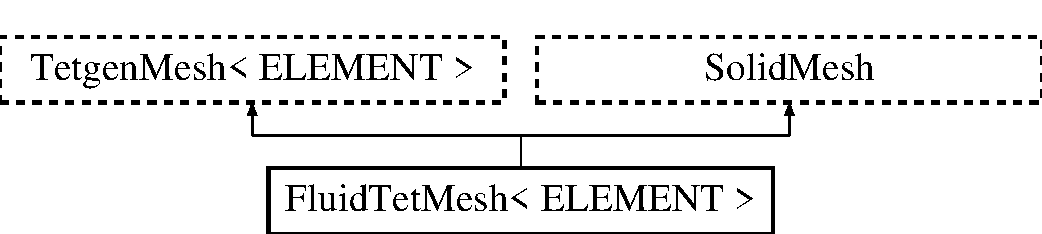
\includegraphics[height=2.000000cm]{classFluidTetMesh}
\end{center}
\end{figure}
\subsection*{Public Member Functions}
\begin{DoxyCompactItemize}
\item 
\hyperlink{classFluidTetMesh_a5f8ea145d68623198abc97209a0491a6}{Fluid\+Tet\+Mesh} (const std\+::string \&node\+\_\+file\+\_\+name, const std\+::string \&element\+\_\+file\+\_\+name, const std\+::string \&face\+\_\+file\+\_\+name, const bool \&split\+\_\+corner\+\_\+elements, Time\+Stepper $\ast$time\+\_\+stepper\+\_\+pt=\&Mesh\+::\+Default\+\_\+\+Time\+Stepper)
\begin{DoxyCompactList}\small\item\em Constructor\+: \end{DoxyCompactList}\item 
virtual \hyperlink{classFluidTetMesh_ae3f6cdb8d95cfe46c8f1fc15dd438b42}{$\sim$\+Fluid\+Tet\+Mesh} ()
\begin{DoxyCompactList}\small\item\em Empty Destructor. \end{DoxyCompactList}\end{DoxyCompactItemize}


\subsection{Detailed Description}
\subsubsection*{template$<$class E\+L\+E\+M\+E\+NT$>$\newline
class Fluid\+Tet\+Mesh$<$ E\+L\+E\+M\+E\+N\+T $>$}

Tetgen-\/based mesh upgraded to become a (pseudo-\/) solid mesh. 

Definition at line 102 of file unstructured\+\_\+three\+\_\+d\+\_\+fsi.\+cc.



\subsection{Constructor \& Destructor Documentation}
\mbox{\Hypertarget{classFluidTetMesh_a5f8ea145d68623198abc97209a0491a6}\label{classFluidTetMesh_a5f8ea145d68623198abc97209a0491a6}} 
\index{Fluid\+Tet\+Mesh@{Fluid\+Tet\+Mesh}!Fluid\+Tet\+Mesh@{Fluid\+Tet\+Mesh}}
\index{Fluid\+Tet\+Mesh@{Fluid\+Tet\+Mesh}!Fluid\+Tet\+Mesh@{Fluid\+Tet\+Mesh}}
\subsubsection{\texorpdfstring{Fluid\+Tet\+Mesh()}{FluidTetMesh()}}
{\footnotesize\ttfamily template$<$class E\+L\+E\+M\+E\+NT$>$ \\
\hyperlink{classFluidTetMesh}{Fluid\+Tet\+Mesh}$<$ E\+L\+E\+M\+E\+NT $>$\+::\hyperlink{classFluidTetMesh}{Fluid\+Tet\+Mesh} (\begin{DoxyParamCaption}\item[{const std\+::string \&}]{node\+\_\+file\+\_\+name,  }\item[{const std\+::string \&}]{element\+\_\+file\+\_\+name,  }\item[{const std\+::string \&}]{face\+\_\+file\+\_\+name,  }\item[{const bool \&}]{split\+\_\+corner\+\_\+elements,  }\item[{Time\+Stepper $\ast$}]{time\+\_\+stepper\+\_\+pt = {\ttfamily \&Mesh\+:\+:Default\+\_\+TimeStepper} }\end{DoxyParamCaption})\hspace{0.3cm}{\ttfamily [inline]}}



Constructor\+: 



Definition at line 109 of file unstructured\+\_\+three\+\_\+d\+\_\+fsi.\+cc.

\mbox{\Hypertarget{classFluidTetMesh_ae3f6cdb8d95cfe46c8f1fc15dd438b42}\label{classFluidTetMesh_ae3f6cdb8d95cfe46c8f1fc15dd438b42}} 
\index{Fluid\+Tet\+Mesh@{Fluid\+Tet\+Mesh}!````~Fluid\+Tet\+Mesh@{$\sim$\+Fluid\+Tet\+Mesh}}
\index{````~Fluid\+Tet\+Mesh@{$\sim$\+Fluid\+Tet\+Mesh}!Fluid\+Tet\+Mesh@{Fluid\+Tet\+Mesh}}
\subsubsection{\texorpdfstring{$\sim$\+Fluid\+Tet\+Mesh()}{~FluidTetMesh()}}
{\footnotesize\ttfamily template$<$class E\+L\+E\+M\+E\+NT$>$ \\
virtual \hyperlink{classFluidTetMesh}{Fluid\+Tet\+Mesh}$<$ E\+L\+E\+M\+E\+NT $>$\+::$\sim$\hyperlink{classFluidTetMesh}{Fluid\+Tet\+Mesh} (\begin{DoxyParamCaption}{ }\end{DoxyParamCaption})\hspace{0.3cm}{\ttfamily [inline]}, {\ttfamily [virtual]}}



Empty Destructor. 



Definition at line 147 of file unstructured\+\_\+three\+\_\+d\+\_\+fsi.\+cc.



The documentation for this class was generated from the following file\+:\begin{DoxyCompactItemize}
\item 
\hyperlink{unstructured__three__d__fsi_8cc}{unstructured\+\_\+three\+\_\+d\+\_\+fsi.\+cc}\end{DoxyCompactItemize}

\hypertarget{classMySolidTetgenMesh}{}\section{My\+Solid\+Tetgen\+Mesh$<$ E\+L\+E\+M\+E\+NT $>$ Class Template Reference}
\label{classMySolidTetgenMesh}\index{My\+Solid\+Tetgen\+Mesh$<$ E\+L\+E\+M\+E\+N\+T $>$@{My\+Solid\+Tetgen\+Mesh$<$ E\+L\+E\+M\+E\+N\+T $>$}}


Tetgen-\/based mesh upgraded to become a solid mesh.  


Inheritance diagram for My\+Solid\+Tetgen\+Mesh$<$ E\+L\+E\+M\+E\+NT $>$\+:\begin{figure}[H]
\begin{center}
\leavevmode
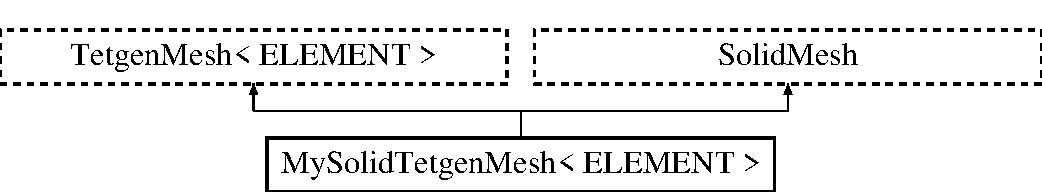
\includegraphics[height=2.000000cm]{classMySolidTetgenMesh}
\end{center}
\end{figure}
\subsection*{Public Member Functions}
\begin{DoxyCompactItemize}
\item 
\hyperlink{classMySolidTetgenMesh_ac6f8d5bf403bb9da0149184c30eb6d8d}{My\+Solid\+Tetgen\+Mesh} (const std\+::string \&node\+\_\+file\+\_\+name, const std\+::string \&element\+\_\+file\+\_\+name, const std\+::string \&face\+\_\+file\+\_\+name, Time\+Stepper $\ast$time\+\_\+stepper\+\_\+pt=\&Mesh\+::\+Default\+\_\+\+Time\+Stepper)
\begin{DoxyCompactList}\small\item\em Constructor\+: \end{DoxyCompactList}\item 
virtual \hyperlink{classMySolidTetgenMesh_ad0e9bf1679a2ba8d3d655b95d7124e91}{$\sim$\+My\+Solid\+Tetgen\+Mesh} ()
\begin{DoxyCompactList}\small\item\em Empty Destructor. \end{DoxyCompactList}\end{DoxyCompactItemize}


\subsection{Detailed Description}
\subsubsection*{template$<$class E\+L\+E\+M\+E\+NT$>$\newline
class My\+Solid\+Tetgen\+Mesh$<$ E\+L\+E\+M\+E\+N\+T $>$}

Tetgen-\/based mesh upgraded to become a solid mesh. 

Definition at line 51 of file unstructured\+\_\+three\+\_\+d\+\_\+solid.\+cc.



\subsection{Constructor \& Destructor Documentation}
\mbox{\Hypertarget{classMySolidTetgenMesh_ac6f8d5bf403bb9da0149184c30eb6d8d}\label{classMySolidTetgenMesh_ac6f8d5bf403bb9da0149184c30eb6d8d}} 
\index{My\+Solid\+Tetgen\+Mesh@{My\+Solid\+Tetgen\+Mesh}!My\+Solid\+Tetgen\+Mesh@{My\+Solid\+Tetgen\+Mesh}}
\index{My\+Solid\+Tetgen\+Mesh@{My\+Solid\+Tetgen\+Mesh}!My\+Solid\+Tetgen\+Mesh@{My\+Solid\+Tetgen\+Mesh}}
\subsubsection{\texorpdfstring{My\+Solid\+Tetgen\+Mesh()}{MySolidTetgenMesh()}}
{\footnotesize\ttfamily template$<$class E\+L\+E\+M\+E\+NT$>$ \\
\hyperlink{classMySolidTetgenMesh}{My\+Solid\+Tetgen\+Mesh}$<$ E\+L\+E\+M\+E\+NT $>$\+::\hyperlink{classMySolidTetgenMesh}{My\+Solid\+Tetgen\+Mesh} (\begin{DoxyParamCaption}\item[{const std\+::string \&}]{node\+\_\+file\+\_\+name,  }\item[{const std\+::string \&}]{element\+\_\+file\+\_\+name,  }\item[{const std\+::string \&}]{face\+\_\+file\+\_\+name,  }\item[{Time\+Stepper $\ast$}]{time\+\_\+stepper\+\_\+pt = {\ttfamily \&Mesh\+:\+:Default\+\_\+TimeStepper} }\end{DoxyParamCaption})\hspace{0.3cm}{\ttfamily [inline]}}



Constructor\+: 



Definition at line 58 of file unstructured\+\_\+three\+\_\+d\+\_\+solid.\+cc.

\mbox{\Hypertarget{classMySolidTetgenMesh_ad0e9bf1679a2ba8d3d655b95d7124e91}\label{classMySolidTetgenMesh_ad0e9bf1679a2ba8d3d655b95d7124e91}} 
\index{My\+Solid\+Tetgen\+Mesh@{My\+Solid\+Tetgen\+Mesh}!````~My\+Solid\+Tetgen\+Mesh@{$\sim$\+My\+Solid\+Tetgen\+Mesh}}
\index{````~My\+Solid\+Tetgen\+Mesh@{$\sim$\+My\+Solid\+Tetgen\+Mesh}!My\+Solid\+Tetgen\+Mesh@{My\+Solid\+Tetgen\+Mesh}}
\subsubsection{\texorpdfstring{$\sim$\+My\+Solid\+Tetgen\+Mesh()}{~MySolidTetgenMesh()}}
{\footnotesize\ttfamily template$<$class E\+L\+E\+M\+E\+NT$>$ \\
virtual \hyperlink{classMySolidTetgenMesh}{My\+Solid\+Tetgen\+Mesh}$<$ E\+L\+E\+M\+E\+NT $>$\+::$\sim$\hyperlink{classMySolidTetgenMesh}{My\+Solid\+Tetgen\+Mesh} (\begin{DoxyParamCaption}{ }\end{DoxyParamCaption})\hspace{0.3cm}{\ttfamily [inline]}, {\ttfamily [virtual]}}



Empty Destructor. 



Definition at line 74 of file unstructured\+\_\+three\+\_\+d\+\_\+solid.\+cc.



The documentation for this class was generated from the following file\+:\begin{DoxyCompactItemize}
\item 
\hyperlink{unstructured__three__d__solid_8cc}{unstructured\+\_\+three\+\_\+d\+\_\+solid.\+cc}\end{DoxyCompactItemize}

\hypertarget{classUnstructuredFSIProblem}{}\section{Unstructured\+F\+S\+I\+Problem$<$ F\+L\+U\+I\+D\+\_\+\+E\+L\+E\+M\+E\+NT, S\+O\+L\+I\+D\+\_\+\+E\+L\+E\+M\+E\+NT $>$ Class Template Reference}
\label{classUnstructuredFSIProblem}\index{Unstructured\+F\+S\+I\+Problem$<$ F\+L\+U\+I\+D\+\_\+\+E\+L\+E\+M\+E\+N\+T, S\+O\+L\+I\+D\+\_\+\+E\+L\+E\+M\+E\+N\+T $>$@{Unstructured\+F\+S\+I\+Problem$<$ F\+L\+U\+I\+D\+\_\+\+E\+L\+E\+M\+E\+N\+T, S\+O\+L\+I\+D\+\_\+\+E\+L\+E\+M\+E\+N\+T $>$}}


Unstructured F\+SI Problem.  


Inheritance diagram for Unstructured\+F\+S\+I\+Problem$<$ F\+L\+U\+I\+D\+\_\+\+E\+L\+E\+M\+E\+NT, S\+O\+L\+I\+D\+\_\+\+E\+L\+E\+M\+E\+NT $>$\+:\begin{figure}[H]
\begin{center}
\leavevmode
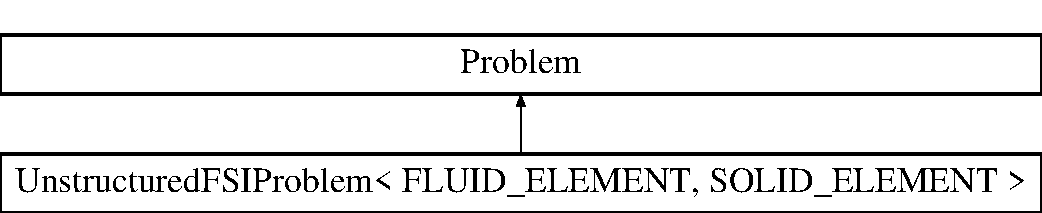
\includegraphics[height=2.000000cm]{classUnstructuredFSIProblem}
\end{center}
\end{figure}
\subsection*{Public Member Functions}
\begin{DoxyCompactItemize}
\item 
\hyperlink{classUnstructuredFSIProblem_a6a31fd839e0215ef1312942cf7284bd2}{Unstructured\+F\+S\+I\+Problem} ()
\begin{DoxyCompactList}\small\item\em Constructor. \end{DoxyCompactList}\item 
\hyperlink{classUnstructuredFSIProblem_a976a81e0dee902f6713bd8ca4d79d000}{$\sim$\+Unstructured\+F\+S\+I\+Problem} ()
\begin{DoxyCompactList}\small\item\em Destructor (empty) \end{DoxyCompactList}\item 
\hyperlink{classFluidTriangleMesh}{Fluid\+Triangle\+Mesh}$<$ F\+L\+U\+I\+D\+\_\+\+E\+L\+E\+M\+E\+NT $>$ $\ast$\& \hyperlink{classUnstructuredFSIProblem_afe86a739cadf57036a0bf351ed9bc1a9}{fluid\+\_\+mesh\+\_\+pt} ()
\begin{DoxyCompactList}\small\item\em Access function for the fluid mesh. \end{DoxyCompactList}\item 
\hyperlink{classMySolidTriangleMesh}{My\+Solid\+Triangle\+Mesh}$<$ S\+O\+L\+I\+D\+\_\+\+E\+L\+E\+M\+E\+NT $>$ $\ast$\& \hyperlink{classUnstructuredFSIProblem_ad1430c627842b8ea0a373adcf571647f}{solid\+\_\+mesh\+\_\+pt} ()
\begin{DoxyCompactList}\small\item\em Access function for the solid mesh. \end{DoxyCompactList}\item 
void \hyperlink{classUnstructuredFSIProblem_a15f581318b505de07f50bd570da8c8d0}{doc\+\_\+solution} (Doc\+Info \&doc\+\_\+info)
\begin{DoxyCompactList}\small\item\em Doc the solution. \end{DoxyCompactList}\end{DoxyCompactItemize}
\subsection*{Private Member Functions}
\begin{DoxyCompactItemize}
\item 
void \hyperlink{classUnstructuredFSIProblem_a934a587c99668fca969a72814b3142a7}{create\+\_\+fsi\+\_\+traction\+\_\+elements} ()
\begin{DoxyCompactList}\small\item\em Create F\+SI traction elements. \end{DoxyCompactList}\item 
void \hyperlink{classUnstructuredFSIProblem_a6f810c300f373cfc79e23d58f95944e3}{create\+\_\+lagrange\+\_\+multiplier\+\_\+elements} ()
\begin{DoxyCompactList}\small\item\em Create elements that enforce prescribed boundary motion for the pseudo-\/solid fluid mesh by Lagrange multipliers. \end{DoxyCompactList}\item 
void \hyperlink{classUnstructuredFSIProblem_a6b86e58ba6cf2871a8e049dd91f6b8b9}{doc\+\_\+solid\+\_\+boundary\+\_\+coordinates} ()
\begin{DoxyCompactList}\small\item\em Sanity check\+: Doc boundary coordinates from solid side. \end{DoxyCompactList}\end{DoxyCompactItemize}
\subsection*{Private Attributes}
\begin{DoxyCompactItemize}
\item 
\hyperlink{classFluidTriangleMesh}{Fluid\+Triangle\+Mesh}$<$ F\+L\+U\+I\+D\+\_\+\+E\+L\+E\+M\+E\+NT $>$ $\ast$ \hyperlink{classUnstructuredFSIProblem_a33c3b4cd9923f8b25368ff20e4810b2c}{Fluid\+\_\+mesh\+\_\+pt}
\begin{DoxyCompactList}\small\item\em Fluid mesh. \end{DoxyCompactList}\item 
\hyperlink{classMySolidTriangleMesh}{My\+Solid\+Triangle\+Mesh}$<$ S\+O\+L\+I\+D\+\_\+\+E\+L\+E\+M\+E\+NT $>$ $\ast$ \hyperlink{classUnstructuredFSIProblem_aeb164665366e237ca311e448466d7c9d}{Solid\+\_\+mesh\+\_\+pt}
\begin{DoxyCompactList}\small\item\em Solid mesh. \end{DoxyCompactList}\item 
Solid\+Mesh $\ast$ \hyperlink{classUnstructuredFSIProblem_ab30c2bc8de791e91d0bba19b048b5219}{Lagrange\+\_\+multiplier\+\_\+mesh\+\_\+pt}
\begin{DoxyCompactList}\small\item\em Pointers to mesh of Lagrange multiplier elements. \end{DoxyCompactList}\item 
Solid\+Mesh $\ast$ \hyperlink{classUnstructuredFSIProblem_ab7ada68f864e990b7b5e40000c289aa1}{Traction\+\_\+mesh\+\_\+pt}
\begin{DoxyCompactList}\small\item\em Vector of pointers to mesh of F\+SI traction elements. \end{DoxyCompactList}\item 
Mesh\+As\+Geom\+Object $\ast$ \hyperlink{classUnstructuredFSIProblem_aa7471e8fb88098faa147e1162480feff}{Solid\+\_\+fsi\+\_\+boundary\+\_\+pt}
\begin{DoxyCompactList}\small\item\em Geom\+Object incarnation of fsi boundary in solid mesh. \end{DoxyCompactList}\end{DoxyCompactItemize}


\subsection{Detailed Description}
\subsubsection*{template$<$class F\+L\+U\+I\+D\+\_\+\+E\+L\+E\+M\+E\+NT, class S\+O\+L\+I\+D\+\_\+\+E\+L\+E\+M\+E\+NT$>$\newline
class Unstructured\+F\+S\+I\+Problem$<$ F\+L\+U\+I\+D\+\_\+\+E\+L\+E\+M\+E\+N\+T, S\+O\+L\+I\+D\+\_\+\+E\+L\+E\+M\+E\+N\+T $>$}

Unstructured F\+SI Problem. 

Definition at line 277 of file unstructured\+\_\+two\+\_\+d\+\_\+fsi.\+cc.



\subsection{Constructor \& Destructor Documentation}
\mbox{\Hypertarget{classUnstructuredFSIProblem_a6a31fd839e0215ef1312942cf7284bd2}\label{classUnstructuredFSIProblem_a6a31fd839e0215ef1312942cf7284bd2}} 
\index{Unstructured\+F\+S\+I\+Problem@{Unstructured\+F\+S\+I\+Problem}!Unstructured\+F\+S\+I\+Problem@{Unstructured\+F\+S\+I\+Problem}}
\index{Unstructured\+F\+S\+I\+Problem@{Unstructured\+F\+S\+I\+Problem}!Unstructured\+F\+S\+I\+Problem@{Unstructured\+F\+S\+I\+Problem}}
\subsubsection{\texorpdfstring{Unstructured\+F\+S\+I\+Problem()}{UnstructuredFSIProblem()}}
{\footnotesize\ttfamily template$<$class F\+L\+U\+I\+D\+\_\+\+E\+L\+E\+M\+E\+NT , class S\+O\+L\+I\+D\+\_\+\+E\+L\+E\+M\+E\+NT $>$ \\
\hyperlink{classUnstructuredFSIProblem}{Unstructured\+F\+S\+I\+Problem}$<$ F\+L\+U\+I\+D\+\_\+\+E\+L\+E\+M\+E\+NT, S\+O\+L\+I\+D\+\_\+\+E\+L\+E\+M\+E\+NT $>$\+::\hyperlink{classUnstructuredFSIProblem}{Unstructured\+F\+S\+I\+Problem} (\begin{DoxyParamCaption}{ }\end{DoxyParamCaption})}



Constructor. 

Constructor for unstructured F\+SI problem. 

Definition at line 339 of file unstructured\+\_\+two\+\_\+d\+\_\+fsi.\+cc.



References Global\+\_\+\+Parameters\+::\+Constitutive\+\_\+law\+\_\+pt, Unstructured\+F\+S\+I\+Problem$<$ F\+L\+U\+I\+D\+\_\+\+E\+L\+E\+M\+E\+N\+T, S\+O\+L\+I\+D\+\_\+\+E\+L\+E\+M\+E\+N\+T $>$\+::doc\+\_\+solid\+\_\+boundary\+\_\+coordinates(), Global\+\_\+\+Parameters\+::gravity(), and Global\+\_\+\+Parameters\+::\+Re.

\mbox{\Hypertarget{classUnstructuredFSIProblem_a976a81e0dee902f6713bd8ca4d79d000}\label{classUnstructuredFSIProblem_a976a81e0dee902f6713bd8ca4d79d000}} 
\index{Unstructured\+F\+S\+I\+Problem@{Unstructured\+F\+S\+I\+Problem}!````~Unstructured\+F\+S\+I\+Problem@{$\sim$\+Unstructured\+F\+S\+I\+Problem}}
\index{````~Unstructured\+F\+S\+I\+Problem@{$\sim$\+Unstructured\+F\+S\+I\+Problem}!Unstructured\+F\+S\+I\+Problem@{Unstructured\+F\+S\+I\+Problem}}
\subsubsection{\texorpdfstring{$\sim$\+Unstructured\+F\+S\+I\+Problem()}{~UnstructuredFSIProblem()}}
{\footnotesize\ttfamily template$<$class F\+L\+U\+I\+D\+\_\+\+E\+L\+E\+M\+E\+NT , class S\+O\+L\+I\+D\+\_\+\+E\+L\+E\+M\+E\+NT $>$ \\
\hyperlink{classUnstructuredFSIProblem}{Unstructured\+F\+S\+I\+Problem}$<$ F\+L\+U\+I\+D\+\_\+\+E\+L\+E\+M\+E\+NT, S\+O\+L\+I\+D\+\_\+\+E\+L\+E\+M\+E\+NT $>$\+::$\sim$\hyperlink{classUnstructuredFSIProblem}{Unstructured\+F\+S\+I\+Problem} (\begin{DoxyParamCaption}{ }\end{DoxyParamCaption})\hspace{0.3cm}{\ttfamily [inline]}}



Destructor (empty) 



Definition at line 286 of file unstructured\+\_\+two\+\_\+d\+\_\+fsi.\+cc.



\subsection{Member Function Documentation}
\mbox{\Hypertarget{classUnstructuredFSIProblem_a934a587c99668fca969a72814b3142a7}\label{classUnstructuredFSIProblem_a934a587c99668fca969a72814b3142a7}} 
\index{Unstructured\+F\+S\+I\+Problem@{Unstructured\+F\+S\+I\+Problem}!create\+\_\+fsi\+\_\+traction\+\_\+elements@{create\+\_\+fsi\+\_\+traction\+\_\+elements}}
\index{create\+\_\+fsi\+\_\+traction\+\_\+elements@{create\+\_\+fsi\+\_\+traction\+\_\+elements}!Unstructured\+F\+S\+I\+Problem@{Unstructured\+F\+S\+I\+Problem}}
\subsubsection{\texorpdfstring{create\+\_\+fsi\+\_\+traction\+\_\+elements()}{create\_fsi\_traction\_elements()}}
{\footnotesize\ttfamily template$<$class F\+L\+U\+I\+D\+\_\+\+E\+L\+E\+M\+E\+NT , class S\+O\+L\+I\+D\+\_\+\+E\+L\+E\+M\+E\+NT $>$ \\
void \hyperlink{classUnstructuredFSIProblem}{Unstructured\+F\+S\+I\+Problem}$<$ F\+L\+U\+I\+D\+\_\+\+E\+L\+E\+M\+E\+NT, S\+O\+L\+I\+D\+\_\+\+E\+L\+E\+M\+E\+NT $>$\+::create\+\_\+fsi\+\_\+traction\+\_\+elements (\begin{DoxyParamCaption}{ }\end{DoxyParamCaption})\hspace{0.3cm}{\ttfamily [private]}}



Create F\+SI traction elements. 



Definition at line 642 of file unstructured\+\_\+two\+\_\+d\+\_\+fsi.\+cc.



References Unstructured\+F\+S\+I\+Problem$<$ F\+L\+U\+I\+D\+\_\+\+E\+L\+E\+M\+E\+N\+T, S\+O\+L\+I\+D\+\_\+\+E\+L\+E\+M\+E\+N\+T $>$\+::create\+\_\+lagrange\+\_\+multiplier\+\_\+elements(), and Global\+\_\+\+Parameters\+::Q.



Referenced by Unstructured\+F\+S\+I\+Problem$<$ F\+L\+U\+I\+D\+\_\+\+E\+L\+E\+M\+E\+N\+T, S\+O\+L\+I\+D\+\_\+\+E\+L\+E\+M\+E\+N\+T $>$\+::doc\+\_\+solid\+\_\+boundary\+\_\+coordinates().

\mbox{\Hypertarget{classUnstructuredFSIProblem_a6f810c300f373cfc79e23d58f95944e3}\label{classUnstructuredFSIProblem_a6f810c300f373cfc79e23d58f95944e3}} 
\index{Unstructured\+F\+S\+I\+Problem@{Unstructured\+F\+S\+I\+Problem}!create\+\_\+lagrange\+\_\+multiplier\+\_\+elements@{create\+\_\+lagrange\+\_\+multiplier\+\_\+elements}}
\index{create\+\_\+lagrange\+\_\+multiplier\+\_\+elements@{create\+\_\+lagrange\+\_\+multiplier\+\_\+elements}!Unstructured\+F\+S\+I\+Problem@{Unstructured\+F\+S\+I\+Problem}}
\subsubsection{\texorpdfstring{create\+\_\+lagrange\+\_\+multiplier\+\_\+elements()}{create\_lagrange\_multiplier\_elements()}}
{\footnotesize\ttfamily template$<$class F\+L\+U\+I\+D\+\_\+\+E\+L\+E\+M\+E\+NT , class S\+O\+L\+I\+D\+\_\+\+E\+L\+E\+M\+E\+NT $>$ \\
void \hyperlink{classUnstructuredFSIProblem}{Unstructured\+F\+S\+I\+Problem}$<$ F\+L\+U\+I\+D\+\_\+\+E\+L\+E\+M\+E\+NT, S\+O\+L\+I\+D\+\_\+\+E\+L\+E\+M\+E\+NT $>$\+::create\+\_\+lagrange\+\_\+multiplier\+\_\+elements (\begin{DoxyParamCaption}{ }\end{DoxyParamCaption})\hspace{0.3cm}{\ttfamily [private]}}



Create elements that enforce prescribed boundary motion for the pseudo-\/solid fluid mesh by Lagrange multipliers. 

Create elements that impose the prescribed boundary displacement for the pseudo-\/solid fluid mesh 

Definition at line 684 of file unstructured\+\_\+two\+\_\+d\+\_\+fsi.\+cc.



References Unstructured\+F\+S\+I\+Problem$<$ F\+L\+U\+I\+D\+\_\+\+E\+L\+E\+M\+E\+N\+T, S\+O\+L\+I\+D\+\_\+\+E\+L\+E\+M\+E\+N\+T $>$\+::doc\+\_\+solution().



Referenced by Unstructured\+F\+S\+I\+Problem$<$ F\+L\+U\+I\+D\+\_\+\+E\+L\+E\+M\+E\+N\+T, S\+O\+L\+I\+D\+\_\+\+E\+L\+E\+M\+E\+N\+T $>$\+::create\+\_\+fsi\+\_\+traction\+\_\+elements().

\mbox{\Hypertarget{classUnstructuredFSIProblem_a6b86e58ba6cf2871a8e049dd91f6b8b9}\label{classUnstructuredFSIProblem_a6b86e58ba6cf2871a8e049dd91f6b8b9}} 
\index{Unstructured\+F\+S\+I\+Problem@{Unstructured\+F\+S\+I\+Problem}!doc\+\_\+solid\+\_\+boundary\+\_\+coordinates@{doc\+\_\+solid\+\_\+boundary\+\_\+coordinates}}
\index{doc\+\_\+solid\+\_\+boundary\+\_\+coordinates@{doc\+\_\+solid\+\_\+boundary\+\_\+coordinates}!Unstructured\+F\+S\+I\+Problem@{Unstructured\+F\+S\+I\+Problem}}
\subsubsection{\texorpdfstring{doc\+\_\+solid\+\_\+boundary\+\_\+coordinates()}{doc\_solid\_boundary\_coordinates()}}
{\footnotesize\ttfamily template$<$class F\+L\+U\+I\+D\+\_\+\+E\+L\+E\+M\+E\+NT , class S\+O\+L\+I\+D\+\_\+\+E\+L\+E\+M\+E\+NT $>$ \\
void \hyperlink{classUnstructuredFSIProblem}{Unstructured\+F\+S\+I\+Problem}$<$ F\+L\+U\+I\+D\+\_\+\+E\+L\+E\+M\+E\+NT, S\+O\+L\+I\+D\+\_\+\+E\+L\+E\+M\+E\+NT $>$\+::doc\+\_\+solid\+\_\+boundary\+\_\+coordinates (\begin{DoxyParamCaption}{ }\end{DoxyParamCaption})\hspace{0.3cm}{\ttfamily [private]}}



Sanity check\+: Doc boundary coordinates from solid side. 

Doc boundary coordinates in solid and plot Geom\+Object representation of F\+SI boundary. 

Definition at line 567 of file unstructured\+\_\+two\+\_\+d\+\_\+fsi.\+cc.



References Unstructured\+F\+S\+I\+Problem$<$ F\+L\+U\+I\+D\+\_\+\+E\+L\+E\+M\+E\+N\+T, S\+O\+L\+I\+D\+\_\+\+E\+L\+E\+M\+E\+N\+T $>$\+::create\+\_\+fsi\+\_\+traction\+\_\+elements().



Referenced by Unstructured\+F\+S\+I\+Problem$<$ F\+L\+U\+I\+D\+\_\+\+E\+L\+E\+M\+E\+N\+T, S\+O\+L\+I\+D\+\_\+\+E\+L\+E\+M\+E\+N\+T $>$\+::\+Unstructured\+F\+S\+I\+Problem().

\mbox{\Hypertarget{classUnstructuredFSIProblem_a15f581318b505de07f50bd570da8c8d0}\label{classUnstructuredFSIProblem_a15f581318b505de07f50bd570da8c8d0}} 
\index{Unstructured\+F\+S\+I\+Problem@{Unstructured\+F\+S\+I\+Problem}!doc\+\_\+solution@{doc\+\_\+solution}}
\index{doc\+\_\+solution@{doc\+\_\+solution}!Unstructured\+F\+S\+I\+Problem@{Unstructured\+F\+S\+I\+Problem}}
\subsubsection{\texorpdfstring{doc\+\_\+solution()}{doc\_solution()}}
{\footnotesize\ttfamily template$<$class F\+L\+U\+I\+D\+\_\+\+E\+L\+E\+M\+E\+NT , class S\+O\+L\+I\+D\+\_\+\+E\+L\+E\+M\+E\+NT $>$ \\
void \hyperlink{classUnstructuredFSIProblem}{Unstructured\+F\+S\+I\+Problem}$<$ F\+L\+U\+I\+D\+\_\+\+E\+L\+E\+M\+E\+NT, S\+O\+L\+I\+D\+\_\+\+E\+L\+E\+M\+E\+NT $>$\+::doc\+\_\+solution (\begin{DoxyParamCaption}\item[{Doc\+Info \&}]{doc\+\_\+info }\end{DoxyParamCaption})}



Doc the solution. 



Definition at line 752 of file unstructured\+\_\+two\+\_\+d\+\_\+fsi.\+cc.



Referenced by Unstructured\+F\+S\+I\+Problem$<$ F\+L\+U\+I\+D\+\_\+\+E\+L\+E\+M\+E\+N\+T, S\+O\+L\+I\+D\+\_\+\+E\+L\+E\+M\+E\+N\+T $>$\+::create\+\_\+lagrange\+\_\+multiplier\+\_\+elements().

\mbox{\Hypertarget{classUnstructuredFSIProblem_afe86a739cadf57036a0bf351ed9bc1a9}\label{classUnstructuredFSIProblem_afe86a739cadf57036a0bf351ed9bc1a9}} 
\index{Unstructured\+F\+S\+I\+Problem@{Unstructured\+F\+S\+I\+Problem}!fluid\+\_\+mesh\+\_\+pt@{fluid\+\_\+mesh\+\_\+pt}}
\index{fluid\+\_\+mesh\+\_\+pt@{fluid\+\_\+mesh\+\_\+pt}!Unstructured\+F\+S\+I\+Problem@{Unstructured\+F\+S\+I\+Problem}}
\subsubsection{\texorpdfstring{fluid\+\_\+mesh\+\_\+pt()}{fluid\_mesh\_pt()}}
{\footnotesize\ttfamily template$<$class F\+L\+U\+I\+D\+\_\+\+E\+L\+E\+M\+E\+NT , class S\+O\+L\+I\+D\+\_\+\+E\+L\+E\+M\+E\+NT $>$ \\
\hyperlink{classFluidTriangleMesh}{Fluid\+Triangle\+Mesh}$<$F\+L\+U\+I\+D\+\_\+\+E\+L\+E\+M\+E\+NT$>$$\ast$\& \hyperlink{classUnstructuredFSIProblem}{Unstructured\+F\+S\+I\+Problem}$<$ F\+L\+U\+I\+D\+\_\+\+E\+L\+E\+M\+E\+NT, S\+O\+L\+I\+D\+\_\+\+E\+L\+E\+M\+E\+NT $>$\+::fluid\+\_\+mesh\+\_\+pt (\begin{DoxyParamCaption}{ }\end{DoxyParamCaption})\hspace{0.3cm}{\ttfamily [inline]}}



Access function for the fluid mesh. 



Definition at line 289 of file unstructured\+\_\+two\+\_\+d\+\_\+fsi.\+cc.



Referenced by main().

\mbox{\Hypertarget{classUnstructuredFSIProblem_ad1430c627842b8ea0a373adcf571647f}\label{classUnstructuredFSIProblem_ad1430c627842b8ea0a373adcf571647f}} 
\index{Unstructured\+F\+S\+I\+Problem@{Unstructured\+F\+S\+I\+Problem}!solid\+\_\+mesh\+\_\+pt@{solid\+\_\+mesh\+\_\+pt}}
\index{solid\+\_\+mesh\+\_\+pt@{solid\+\_\+mesh\+\_\+pt}!Unstructured\+F\+S\+I\+Problem@{Unstructured\+F\+S\+I\+Problem}}
\subsubsection{\texorpdfstring{solid\+\_\+mesh\+\_\+pt()}{solid\_mesh\_pt()}}
{\footnotesize\ttfamily template$<$class F\+L\+U\+I\+D\+\_\+\+E\+L\+E\+M\+E\+NT , class S\+O\+L\+I\+D\+\_\+\+E\+L\+E\+M\+E\+NT $>$ \\
\hyperlink{classMySolidTriangleMesh}{My\+Solid\+Triangle\+Mesh}$<$S\+O\+L\+I\+D\+\_\+\+E\+L\+E\+M\+E\+NT$>$$\ast$\& \hyperlink{classUnstructuredFSIProblem}{Unstructured\+F\+S\+I\+Problem}$<$ F\+L\+U\+I\+D\+\_\+\+E\+L\+E\+M\+E\+NT, S\+O\+L\+I\+D\+\_\+\+E\+L\+E\+M\+E\+NT $>$\+::solid\+\_\+mesh\+\_\+pt (\begin{DoxyParamCaption}{ }\end{DoxyParamCaption})\hspace{0.3cm}{\ttfamily [inline]}}



Access function for the solid mesh. 



Definition at line 295 of file unstructured\+\_\+two\+\_\+d\+\_\+fsi.\+cc.



\subsection{Member Data Documentation}
\mbox{\Hypertarget{classUnstructuredFSIProblem_a33c3b4cd9923f8b25368ff20e4810b2c}\label{classUnstructuredFSIProblem_a33c3b4cd9923f8b25368ff20e4810b2c}} 
\index{Unstructured\+F\+S\+I\+Problem@{Unstructured\+F\+S\+I\+Problem}!Fluid\+\_\+mesh\+\_\+pt@{Fluid\+\_\+mesh\+\_\+pt}}
\index{Fluid\+\_\+mesh\+\_\+pt@{Fluid\+\_\+mesh\+\_\+pt}!Unstructured\+F\+S\+I\+Problem@{Unstructured\+F\+S\+I\+Problem}}
\subsubsection{\texorpdfstring{Fluid\+\_\+mesh\+\_\+pt}{Fluid\_mesh\_pt}}
{\footnotesize\ttfamily template$<$class F\+L\+U\+I\+D\+\_\+\+E\+L\+E\+M\+E\+NT , class S\+O\+L\+I\+D\+\_\+\+E\+L\+E\+M\+E\+NT $>$ \\
\hyperlink{classFluidTriangleMesh}{Fluid\+Triangle\+Mesh}$<$F\+L\+U\+I\+D\+\_\+\+E\+L\+E\+M\+E\+NT$>$$\ast$ \hyperlink{classUnstructuredFSIProblem}{Unstructured\+F\+S\+I\+Problem}$<$ F\+L\+U\+I\+D\+\_\+\+E\+L\+E\+M\+E\+NT, S\+O\+L\+I\+D\+\_\+\+E\+L\+E\+M\+E\+NT $>$\+::Fluid\+\_\+mesh\+\_\+pt\hspace{0.3cm}{\ttfamily [private]}}



Fluid mesh. 



Definition at line 316 of file unstructured\+\_\+two\+\_\+d\+\_\+fsi.\+cc.

\mbox{\Hypertarget{classUnstructuredFSIProblem_ab30c2bc8de791e91d0bba19b048b5219}\label{classUnstructuredFSIProblem_ab30c2bc8de791e91d0bba19b048b5219}} 
\index{Unstructured\+F\+S\+I\+Problem@{Unstructured\+F\+S\+I\+Problem}!Lagrange\+\_\+multiplier\+\_\+mesh\+\_\+pt@{Lagrange\+\_\+multiplier\+\_\+mesh\+\_\+pt}}
\index{Lagrange\+\_\+multiplier\+\_\+mesh\+\_\+pt@{Lagrange\+\_\+multiplier\+\_\+mesh\+\_\+pt}!Unstructured\+F\+S\+I\+Problem@{Unstructured\+F\+S\+I\+Problem}}
\subsubsection{\texorpdfstring{Lagrange\+\_\+multiplier\+\_\+mesh\+\_\+pt}{Lagrange\_multiplier\_mesh\_pt}}
{\footnotesize\ttfamily template$<$class F\+L\+U\+I\+D\+\_\+\+E\+L\+E\+M\+E\+NT , class S\+O\+L\+I\+D\+\_\+\+E\+L\+E\+M\+E\+NT $>$ \\
Solid\+Mesh$\ast$ \hyperlink{classUnstructuredFSIProblem}{Unstructured\+F\+S\+I\+Problem}$<$ F\+L\+U\+I\+D\+\_\+\+E\+L\+E\+M\+E\+NT, S\+O\+L\+I\+D\+\_\+\+E\+L\+E\+M\+E\+NT $>$\+::Lagrange\+\_\+multiplier\+\_\+mesh\+\_\+pt\hspace{0.3cm}{\ttfamily [private]}}



Pointers to mesh of Lagrange multiplier elements. 



Definition at line 322 of file unstructured\+\_\+two\+\_\+d\+\_\+fsi.\+cc.

\mbox{\Hypertarget{classUnstructuredFSIProblem_aa7471e8fb88098faa147e1162480feff}\label{classUnstructuredFSIProblem_aa7471e8fb88098faa147e1162480feff}} 
\index{Unstructured\+F\+S\+I\+Problem@{Unstructured\+F\+S\+I\+Problem}!Solid\+\_\+fsi\+\_\+boundary\+\_\+pt@{Solid\+\_\+fsi\+\_\+boundary\+\_\+pt}}
\index{Solid\+\_\+fsi\+\_\+boundary\+\_\+pt@{Solid\+\_\+fsi\+\_\+boundary\+\_\+pt}!Unstructured\+F\+S\+I\+Problem@{Unstructured\+F\+S\+I\+Problem}}
\subsubsection{\texorpdfstring{Solid\+\_\+fsi\+\_\+boundary\+\_\+pt}{Solid\_fsi\_boundary\_pt}}
{\footnotesize\ttfamily template$<$class F\+L\+U\+I\+D\+\_\+\+E\+L\+E\+M\+E\+NT , class S\+O\+L\+I\+D\+\_\+\+E\+L\+E\+M\+E\+NT $>$ \\
Mesh\+As\+Geom\+Object$\ast$ \hyperlink{classUnstructuredFSIProblem}{Unstructured\+F\+S\+I\+Problem}$<$ F\+L\+U\+I\+D\+\_\+\+E\+L\+E\+M\+E\+NT, S\+O\+L\+I\+D\+\_\+\+E\+L\+E\+M\+E\+NT $>$\+::Solid\+\_\+fsi\+\_\+boundary\+\_\+pt\hspace{0.3cm}{\ttfamily [private]}}



Geom\+Object incarnation of fsi boundary in solid mesh. 



Definition at line 329 of file unstructured\+\_\+two\+\_\+d\+\_\+fsi.\+cc.

\mbox{\Hypertarget{classUnstructuredFSIProblem_aeb164665366e237ca311e448466d7c9d}\label{classUnstructuredFSIProblem_aeb164665366e237ca311e448466d7c9d}} 
\index{Unstructured\+F\+S\+I\+Problem@{Unstructured\+F\+S\+I\+Problem}!Solid\+\_\+mesh\+\_\+pt@{Solid\+\_\+mesh\+\_\+pt}}
\index{Solid\+\_\+mesh\+\_\+pt@{Solid\+\_\+mesh\+\_\+pt}!Unstructured\+F\+S\+I\+Problem@{Unstructured\+F\+S\+I\+Problem}}
\subsubsection{\texorpdfstring{Solid\+\_\+mesh\+\_\+pt}{Solid\_mesh\_pt}}
{\footnotesize\ttfamily template$<$class F\+L\+U\+I\+D\+\_\+\+E\+L\+E\+M\+E\+NT , class S\+O\+L\+I\+D\+\_\+\+E\+L\+E\+M\+E\+NT $>$ \\
\hyperlink{classMySolidTriangleMesh}{My\+Solid\+Triangle\+Mesh}$<$S\+O\+L\+I\+D\+\_\+\+E\+L\+E\+M\+E\+NT$>$$\ast$ \hyperlink{classUnstructuredFSIProblem}{Unstructured\+F\+S\+I\+Problem}$<$ F\+L\+U\+I\+D\+\_\+\+E\+L\+E\+M\+E\+NT, S\+O\+L\+I\+D\+\_\+\+E\+L\+E\+M\+E\+NT $>$\+::Solid\+\_\+mesh\+\_\+pt\hspace{0.3cm}{\ttfamily [private]}}



Solid mesh. 



Definition at line 319 of file unstructured\+\_\+two\+\_\+d\+\_\+fsi.\+cc.

\mbox{\Hypertarget{classUnstructuredFSIProblem_ab7ada68f864e990b7b5e40000c289aa1}\label{classUnstructuredFSIProblem_ab7ada68f864e990b7b5e40000c289aa1}} 
\index{Unstructured\+F\+S\+I\+Problem@{Unstructured\+F\+S\+I\+Problem}!Traction\+\_\+mesh\+\_\+pt@{Traction\+\_\+mesh\+\_\+pt}}
\index{Traction\+\_\+mesh\+\_\+pt@{Traction\+\_\+mesh\+\_\+pt}!Unstructured\+F\+S\+I\+Problem@{Unstructured\+F\+S\+I\+Problem}}
\subsubsection{\texorpdfstring{Traction\+\_\+mesh\+\_\+pt}{Traction\_mesh\_pt}}
{\footnotesize\ttfamily template$<$class F\+L\+U\+I\+D\+\_\+\+E\+L\+E\+M\+E\+NT , class S\+O\+L\+I\+D\+\_\+\+E\+L\+E\+M\+E\+NT $>$ \\
Solid\+Mesh$\ast$ \hyperlink{classUnstructuredFSIProblem}{Unstructured\+F\+S\+I\+Problem}$<$ F\+L\+U\+I\+D\+\_\+\+E\+L\+E\+M\+E\+NT, S\+O\+L\+I\+D\+\_\+\+E\+L\+E\+M\+E\+NT $>$\+::Traction\+\_\+mesh\+\_\+pt\hspace{0.3cm}{\ttfamily [private]}}



Vector of pointers to mesh of F\+SI traction elements. 



Definition at line 325 of file unstructured\+\_\+two\+\_\+d\+\_\+fsi.\+cc.



The documentation for this class was generated from the following file\+:\begin{DoxyCompactItemize}
\item 
\hyperlink{unstructured__two__d__fsi_8cc}{unstructured\+\_\+two\+\_\+d\+\_\+fsi.\+cc}\end{DoxyCompactItemize}

\chapter{File Documentation}
\hypertarget{unstructured__three__d__fsi_8cc}{}\section{unstructured\+\_\+three\+\_\+d\+\_\+fsi.\+cc File Reference}
\label{unstructured__three__d__fsi_8cc}\index{unstructured\+\_\+three\+\_\+d\+\_\+fsi.\+cc@{unstructured\+\_\+three\+\_\+d\+\_\+fsi.\+cc}}
\subsection*{Classes}
\begin{DoxyCompactItemize}
\item 
class \hyperlink{classMySolidTetgenMesh}{My\+Solid\+Tetgen\+Mesh$<$ E\+L\+E\+M\+E\+N\+T $>$}
\begin{DoxyCompactList}\small\item\em Tetgen-\/based mesh upgraded to become a solid mesh. \end{DoxyCompactList}\item 
class \hyperlink{classFluidTetMesh}{Fluid\+Tet\+Mesh$<$ E\+L\+E\+M\+E\+N\+T $>$}
\begin{DoxyCompactList}\small\item\em Tetgen-\/based mesh upgraded to become a (pseudo-\/) solid mesh. \end{DoxyCompactList}\item 
class \hyperlink{classUnstructuredFSIProblem}{Unstructured\+F\+S\+I\+Problem$<$ F\+L\+U\+I\+D\+\_\+\+E\+L\+E\+M\+E\+N\+T, S\+O\+L\+I\+D\+\_\+\+E\+L\+E\+M\+E\+N\+T $>$}
\begin{DoxyCompactList}\small\item\em Unstructured 3D F\+SI problem. \end{DoxyCompactList}\end{DoxyCompactItemize}
\subsection*{Namespaces}
\begin{DoxyCompactItemize}
\item 
 \hyperlink{namespaceGlobal__Parameters}{Global\+\_\+\+Parameters}
\begin{DoxyCompactList}\small\item\em Global variables. \end{DoxyCompactList}\end{DoxyCompactItemize}
\subsection*{Functions}
\begin{DoxyCompactItemize}
\item 
void \hyperlink{namespaceGlobal__Parameters_af7faf65214ed9ead637f7c208addb095}{Global\+\_\+\+Parameters\+::prescribed\+\_\+inflow\+\_\+traction} (const double \&t, const Vector$<$ double $>$ \&x, const Vector$<$ double $>$ \&n, Vector$<$ double $>$ \&traction)
\begin{DoxyCompactList}\small\item\em Applied traction on fluid at the inflow boundary. \end{DoxyCompactList}\item 
void \hyperlink{namespaceGlobal__Parameters_a83155358b144cff7e29ecb6b209a2d3e}{Global\+\_\+\+Parameters\+::prescribed\+\_\+outflow\+\_\+traction} (const double \&t, const Vector$<$ double $>$ \&x, const Vector$<$ double $>$ \&n, Vector$<$ double $>$ \&traction)
\begin{DoxyCompactList}\small\item\em Applied traction on fluid at the inflow boundary. \end{DoxyCompactList}\item 
int \hyperlink{unstructured__three__d__fsi_8cc_a3c04138a5bfe5d72780bb7e82a18e627}{main} (int argc, char $\ast$$\ast$argv)
\begin{DoxyCompactList}\small\item\em Demonstrate how to solve an unstructured 3D F\+SI problem. \end{DoxyCompactList}\end{DoxyCompactItemize}
\subsection*{Variables}
\begin{DoxyCompactItemize}
\item 
double \hyperlink{namespaceGlobal__Parameters_a9d72e94a9305c6a310940a6a427ebe06}{Global\+\_\+\+Parameters\+::\+Re} =100.\+0
\begin{DoxyCompactList}\small\item\em Default Reynolds number. \end{DoxyCompactList}\item 
double \hyperlink{namespaceGlobal__Parameters_a7814fddf663e56168174a42d2cd6b4c1}{Global\+\_\+\+Parameters\+::Q} =0.\+0
\begin{DoxyCompactList}\small\item\em Default F\+SI parameter. \end{DoxyCompactList}\item 
Constitutive\+Law $\ast$ \hyperlink{namespaceGlobal__Parameters_adbd1f040f375c96fe56b3f475f7dbec2}{Global\+\_\+\+Parameters\+::\+Constitutive\+\_\+law\+\_\+pt} =0
\begin{DoxyCompactList}\small\item\em Pointer to constitutive law. \end{DoxyCompactList}\item 
double \hyperlink{namespaceGlobal__Parameters_a20fccdcfa2c15ad8b951b9ada3bb1661}{Global\+\_\+\+Parameters\+::\+Nu} =0.\+3
\begin{DoxyCompactList}\small\item\em Poisson\textquotesingle{}s ratio for generalised Hookean constitutive equation. \end{DoxyCompactList}\item 
double \hyperlink{namespaceGlobal__Parameters_a05b26d00935600b5e0149872844f224c}{Global\+\_\+\+Parameters\+::\+P\+\_\+in} =0.\+5
\begin{DoxyCompactList}\small\item\em Fluid pressure on inflow boundary. \end{DoxyCompactList}\item 
double \hyperlink{namespaceGlobal__Parameters_ac680ed856897793d54c9c867da19169c}{Global\+\_\+\+Parameters\+::\+P\+\_\+out} =-\/0.\+5
\begin{DoxyCompactList}\small\item\em Fluid pressure on outflow boundary. \end{DoxyCompactList}\end{DoxyCompactItemize}


\subsection{Function Documentation}
\mbox{\Hypertarget{unstructured__three__d__fsi_8cc_a3c04138a5bfe5d72780bb7e82a18e627}\label{unstructured__three__d__fsi_8cc_a3c04138a5bfe5d72780bb7e82a18e627}} 
\index{unstructured\+\_\+three\+\_\+d\+\_\+fsi.\+cc@{unstructured\+\_\+three\+\_\+d\+\_\+fsi.\+cc}!main@{main}}
\index{main@{main}!unstructured\+\_\+three\+\_\+d\+\_\+fsi.\+cc@{unstructured\+\_\+three\+\_\+d\+\_\+fsi.\+cc}}
\subsubsection{\texorpdfstring{main()}{main()}}
{\footnotesize\ttfamily int main (\begin{DoxyParamCaption}\item[{int}]{argc,  }\item[{char $\ast$$\ast$}]{argv }\end{DoxyParamCaption})}



Demonstrate how to solve an unstructured 3D F\+SI problem. 



Definition at line 1006 of file unstructured\+\_\+three\+\_\+d\+\_\+fsi.\+cc.



References Global\+\_\+\+Parameters\+::\+Constitutive\+\_\+law\+\_\+pt, Unstructured\+F\+S\+I\+Problem$<$ F\+L\+U\+I\+D\+\_\+\+E\+L\+E\+M\+E\+N\+T, S\+O\+L\+I\+D\+\_\+\+E\+L\+E\+M\+E\+N\+T $>$\+::doc\+\_\+solution(), Global\+\_\+\+Parameters\+::\+Nu, and Global\+\_\+\+Parameters\+::Q.


\hypertarget{unstructured__three__d__fsi_8txt__doxygenified_8h}{}\section{unstructured\+\_\+three\+\_\+d\+\_\+fsi.\+txt\+\_\+doxygenified.\+h File Reference}
\label{unstructured__three__d__fsi_8txt__doxygenified_8h}\index{unstructured\+\_\+three\+\_\+d\+\_\+fsi.\+txt\+\_\+doxygenified.\+h@{unstructured\+\_\+three\+\_\+d\+\_\+fsi.\+txt\+\_\+doxygenified.\+h}}

%--- End generated contents ---

% Index
\backmatter
\newpage
\phantomsection
\clearemptydoublepage
\addcontentsline{toc}{chapter}{Index}
\printindex

\end{document}
